\chapter{Binary Classiciation at the Top}\label{chap: framework}

In the previous chapter, we introduced the general formulation of the binary classification problem~\eqref{eq: Binary classification counts} and basic ways how to evaluate the performance of binary classification. Furthermore, we introduced three problems that are closely related to binary classification, but focus on specific performance criteria. Namely: accuracy at the top, ranking problems and problem of hypothesis testing. Eventhough these problems are usually considered separately, they have one important thing in common: all three problems can be formulated as a minimization of the number of misclassified samples below (or above) a certain threshold. More specifically, in the rest of the chapter we show, that all mentioned problems falls into the following unified framework
\begin{mini}{\bm{w}}{
  \lambda_1 \cdot \fp(\bm{s}, t) + \lambda_2 \cdot \fn(\bm{s}, t)
}{\label{eq: aatp counts}}{}
  \addConstraint{s_i}{= f(\bm{x}_i; \bm{w}), \quad}{i \in \I}
  \addConstraint{t}{= G(\Brac[c]{\bm{s}_i; y_i}_{i \in \I}),}
\end{mini}
where function~$G \colon \R^n \times \{0, 1\}^n \to \R$ takes the scores and labels of all samples and computes the decision threshold. In other words, all mentioned problems can be formulated as a binary classification problem with special condition on the decision threshold. Then the problems only differ in the way they define the function~$G$. The important distinction from standard binary classification is that the decision threshold is no longer fixed (as in case of neural networks) or trained independently (as in case of SVM), but is a function of scores of all samples. Therefore, the minimization in the problem~\eqref{eq: aatp counts} is performed only with respect to the one variable~$\bm{w}$.

The problem~\eqref{eq: aatp counts} is difficult to handle, since the objective function contains Iverson function~\eqref{eq: iverson} and therefore is discontinuous. The usual approach how to get a continuous objective function is to employ a surrogate function to replace the Iverson function~\cite{li2014top, grill2016learning}.

\begin{notation}[Surrogate function]\label{not: surrogates}
  In the text below, the symbol~$l$ denotes any convex non-negative non-decreasing function with~$l(0) = 1$. As examples of such function we can mention the hinge loss function or the quadratic hinge loss functions defined as follows
  \begin{equation*}
    \begin{aligned}
      l_{\text{hinge}}(s) & = \max\Brac[c]{0, 1 + s}, \\
      l_{\text{quadratic}}(s) & = \Brac{\max\Brac[c]{0, 1 + s}}^2.\\
    \end{aligned}
  \end{equation*}
  We also use parameter~$\vartheta > 0$ to scale inputs to the surrogate functions.
\end{notation}

Figure~\ref{fig: surrogates} compares Iverson function with hinge loss and quadratic hinge loss with different scaling parameters. As can be seen, the surrogate function always provides an upper approximation of the Iverson function, i.e.~$l(s) \ge \Iverson{s \ge 0}$ for all~$s \in \R.$ Besides that, if the scaling parameter is larger than 1, then the surrogate functions approximate the Iverson function better on the interval~$(-\infty, 0]$. However, the approximation on the interval~$[0, \infty)$ is worse. Even though the scaling parameter affects a lot the quality of the approximation, the usual choice is 1.

\begin{figure}[t]
  \centering
  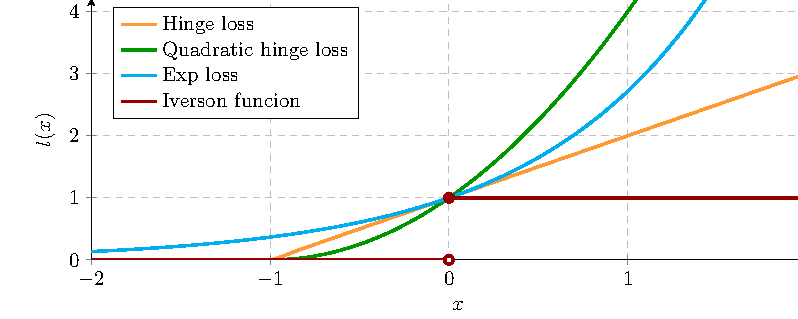
\includegraphics[width = \linewidth]{images/surrogates.pdf}
  \caption{Surrogates}
  \label{fig: surrogates}
\end{figure}

To follow the notation from the previous chapter, we define surrogate approximations of the counts defined in equation~\eqref{eq: confusion counts}. Using surrogate function~$l$ that fulfill the requirements mentioned in Notation~\ref{not: surrogates}, the counts~\eqref{eq: confusion counts} may be approximated by their surrogate counterparts defined as follows
\begin{equation}\label{eq: confusion counts surrogate}
  \begin{aligned}
    \tps(\bm{s}, t) & = \sum_{i \in \Ipos}l(s_i - t), & \qquad
    \fns(\bm{s}, t) & = \sum_{i \in \Ipos}l(t - s_i), \\
    \tns(\bm{s}, t) & = \sum_{i \in \Ineg}l(t - s_i), &
    \fps(\bm{s}, t) & = \sum_{i \in \Ineg}l(s_i - t).
  \end{aligned}
\end{equation}
Since the surrogate function provides upper approximation of the Iverson function, the surrogate counts~\eqref{eq: confusion counts surrogate} provide upper approximations of the true counts~\eqref{eq: confusion counts}. Replacing the counts in~\eqref{eq: aatp counts} by their surrogate counterparts and adding a regularization results in
\begin{mini}{\bm{w}}{
  \frac{\lambda_0}{2} \norm{\bm{w}}^2 + \lambda_1 \cdot \fps(\bm{s}, t) + \lambda_2 \cdot \fns(\bm{s}, t)
  }{\label{eq: aatp surrogate}}{}
  \addConstraint{s_i}{= f(\bm{x}_i; \bm{w}), \quad i \in \I}
  \addConstraint{t}{= G(\Brac[c]{\bm{s}_i; y_i}_{i \in \I}).}
\end{mini}
The regularization is not necessary, but it is usually added for better numerical stability. The resulting optimization problem is easier to solve than problem~\eqref{eq: aatp counts} since the objective function is continuous. To derive other theoretical properties, we need to know the concrete form of the decision threshold function~$G$ as well as the form of the used model~$f.$ Different forms of the function~$G$ are discussed in the rest of this chapter and different forms of model~$f$ in Chapters~\ref{chap: linear} - \ref{chap: deep}.

In the rest of the chapter, we show, that accuracy at the top, ranking problems and the problem of hypothesis testing can be formulated in such a way, that fall  into our general framework of~\eqref{eq: aatp counts} or to its surrogate approximation~\eqref{eq: aatp surrogate}. Most of the problems that we refer to are originally defined for the linear model only, i.e. for~$f(\bm{x}; \bm{w}) = \bm{w}^{\top} \bm{x}.$ However, we formulate all the problems for general model~$f$ and then in Chapters~\ref{chap: linear} - \ref{chap: deep} we discuss their properties based on the used model. 

\begin{notation}[Classification scores]\label{not: scores}
  In Notation~\ref{not: classifier}, we defined vector~$\bm{s} \in \R^n$ of scores of all samples with components defined as
  \begin{equation*}
    s_i = f(\bm{x}_i; \bm{w}), \quad i \in \I,
  \end{equation*}
  where~$f \colon \R^d \to \R$ represents arbitrary model. To simplify the upcoming sections, we define sorted version of the vector of scores~$\bm{s}_{[\cdot]}$ with decreasing components, i.e.
  \begin{equation*}
    s_{[1]}   \ge s_{[2]} \ge \dots \ge s_{[n - 1]} \ge s_{[n]}.
  \end{equation*}
  Similarly, we define vectors~$\bm{s}^- \in \R^{\nneg},$ $\bm{s}^+ \in \R^{\npos}$ of scores of all positive and negative samples with components defined as
  \begin{equation*}
    \begin{aligned}
      s^-_i & = f(\bm{x}_i; \bm{w}), \quad i \in \Ineg, \\
      s^+_i & = f(\bm{x}_i; \bm{w}), \quad i \in \Ipos,
    \end{aligned}
  \end{equation*}
  and their sorted versions~$\bm{s}^-_{[\cdot]}$, $\bm{s}^+_{[\cdot]}$ with decreasing components.
\end{notation}

\section{Ranking problems}\label{sec: ranking}

The first category of formulations falling into our framework~\eqref{eq: aatp counts} and~\eqref{eq: aatp surrogate} are ranking methods which attempt to put as many positive (relevant) samples to the top as possible. The number of positive samples on top equals to the number of positive samples with classification score equal or larger than the highest classicication score corresponding to negative sample. This amounts to maximizing the number of true-positive samples or, equivalently, minimizing the number of false-negative negative samples, which may be written as
\begin{mini}{\bm{w}}{
  \frac{1}{\npos} \fn(\bm{s}, t)
  }{\label{eq: toppush}}{}
  \addConstraint{s_i}{= f(\bm{x}_i; \bm{w}), \quad i \in \I}
  \addConstraint{t}{= s_{[1]}^-}
\end{mini}
Since the threshold~$t$ is a function of score, the problem~\eqref{eq: toppush} is a special case of~\eqref{eq: aatp counts} for~$\lambda_1 = 0$ and~$\lambda_2 = \nicefrac{1}{\npos}$. The authors in~\cite{li2014top} proposed an efficient method to solve the formulation above and called it \TopPush. They replaced the number of false-negative samples with its surrogate counterpart in the objective function of~\eqref{eq: toppush} and added the regularization term to arrive at
\begin{mini}{\bm{w}}{
  \frac{\lambda_0}{2} \norm{\bm{w}}^2 + \frac{1}{\npos} \fns(\bm{s}, t)
  }{\label{eq: toppush surrogate}}{}
  \addConstraint{s_i}{= f(\bm{x}_i; \bm{w}), \quad i \in \I}
  \addConstraint{t}{= s_{[1]}^-}
\end{mini}
Similarly to the original problem, this surrogate approximation falls into our framework of~\eqref{eq: aatp surrogate} for~$\lambda_1 = 0$ and~$\lambda_2 = \nicefrac{1}{\npos}$. However, \TopPush can be very sensitive to outliers. Especially when the linear model is used, as shown in Section~\ref{sec: stability}. To robustify \TopPush formulation, we follow the idea from~\cite{lapin2015top} and propose to replace the largest negative score by the mean of~$K$ largest negative scores. We call this approach \TopPushK and the resulting formulation is as follows
\begin{mini}{\bm{w}}{
  \frac{\lambda_0}{2} \norm{\bm{w}}^2 + \frac{1}{\npos} \fns(\bm{s}, t)
  }{\label{eq: toppushK surrogate}}{}
  \addConstraint{s_i}{= f(\bm{x}_i; \bm{w}), \quad i \in \I}
  \addConstraint{t}{= \sum_{i = 1}^{K} s_{[i]}^-},
\end{mini}
where we use Notation~\ref{not: scores}. We used the mean of highest~$K$ negative scores instead of the value of the~$K$-th negative score to preserve convexity as shown in Section~\ref{sec: convexity}. 

\section{Accuracy at the Top}\label{sec: aatp}

The previous category considers formulations which minimize the number of positive samples below the highest-ranked negative sample, i.e. minimize the number of false-negative samples. Accuracy at the Top~\cite{boyd2012accuracy} takes a different approach and minimizes the number of negative samples with the score above the top~$\tau$-quantile of all scores defined by
\begin{equation}\label{eq: aatp quantile} 
  t_1(\bm{s})
    = \max \Set{t}{\frac{1}{n} \sum_{i \in \I} \Iverson{s_i \ge t} \ge \tau}.
\end{equation}
Then the Accuracy at the Top problem is defined by
\begin{mini}{\bm{w}}{
  \frac{1}{\nneg} \fp(\bm{s}, t)
  }{\label{eq: aatp original}}{}
  \addConstraint{s_i}{= f(\bm{x}_i; \bm{w}), \quad i \in \I}
  \addConstraint{t}{= \max \Set{t}{\frac{1}{n} \sum_{i \in \I} \Iverson{s_i \ge t} \ge \tau}}{~}
\end{mini}
This formulation already falls into our framework~~\eqref{eq: aatp counts} for~$\lambda_1 = \nicefrac{1}{\nneg}$ and~$\lambda_2 = 0$. However, this formulation can be rewritten using the following lemma.
\begin{restatable}{lemma}{lemmaequivalence}\label{lemma:fnfp_equivalence}
  Denote by~$t$ the exact quantile from~\eqref{eq: aatp quantile}. Then for all~$\mu \in [0,1]$ we have
  \begin{equation}\label{eq: fn fp equivalence}
      \fp(\bm{s},t) = \mu \fp(\bm{s},t) + (1-\mu)\fn(\bm{s},t) + (1-\mu)(n\tau - \npos) + (1-\mu)(q - 1),
  \end{equation}
  where~$q$ represents the number of samples which score is equal to~$t$
  \begin{equation*}
      q := \# \Set{i \in \I}{ \bm{s}_i = t}.
  \end{equation*}
\end{restatable}
\noindent The previous lemma can be used to replace the objective function in~\ref{eq: aatp original}. The right-hand side of~\eqref{eq: fn fp equivalence} consists of three parts. The first one is a convex combination of false-positive and false-negative counts. The second one is a constant term which has no impact on optimization. Finally, the third term~$(1-\mu)\Brac{q - 1}$ equals the number of samples for which their score equals the quantile. However, this term is small in comparison with the true-positive and the false-negative counts and can be neglected. Moreover, when the data are ``truly'' random such as when measurement errors are present, then~$q = 1$ and this term vanishes completely. Altogether, we get the following (almost) equivalent formulation to the problem~\eqref{eq: aatp original}
\begin{mini}{\bm{w}}{
  \mu \fp(\bm{s},t) + (1 - \mu)\fn(\bm{s},t)
  }{\label{eq: aatp original combination}}{}
  \addConstraint{s_i}{= f(\bm{x}_i; \bm{w}), \quad i \in \I}
  \addConstraint{t}{= \max \Set{t}{\frac{1}{n} \sum_{i \in \I} \Iverson{s_i \ge t} \ge \tau},}{~}
\end{mini}
where~$\mu \in [0,1]$. This problem with~$\mu = 0$ equals to~\eqref{eq: aatp original}, while with~$\mu = \nicefrac{\nneg}{n}$ it corresponds to the original definition (without regularization) from~\cite{boyd2012accuracy}.

Paper~\cite{grill2016learning} builds on the Accuracy at the Top problem~\eqref{eq: aatp original combination}, where it replaces false-positive and false-negative counts in the objective function by their surrogate counterparts. This leads to
\begin{mini}{\bm{w}}{
  \frac{\lambda_0}{2} \norm{\bm{w}}^2 + \frac{1}{\nneg}\fps(\bm{s}, t) + \frac{1}{\npos} \fns(\bm{s}, t)
  }{\label{eq: grill}}{}
  \addConstraint{s_i}{= f(\bm{x}_i; \bm{w}), \quad i \in \I}
  \addConstraint{t}{= \max \Set{t}{\frac{1}{n} \sum_{i \in \I} \Iverson{s_i \ge t} \ge \tau}.}{~}
\end{mini}
Based on the first author, we name this formulation \Grill. This formulation falls into our framework~\eqref{eq: aatp surrogate} for~$\lambda_1 = \nicefrac{1}{\nneg}$ and~$\lambda_2 = \nicefrac{1}{\npos}$.

Apart from the quantile~\eqref{eq: aatp quantile}, there are two other possible choices of the threshold. The first on is simple approximation of the the true quantile by mean of the~$n\tau$ largest scores 
\begin{equation}\label{eq: aatp quantile mean} 
  t_2(\bm{s}) = \frac{1}{n\tau} \sum_{i=1}^{n\tau} s_{[i]}.
\end{equation}
where for simplicity we assume, that~$n\tau$ is an integer. The quantile~\eqref{eq: aatp quantile} is sometimes denoted as VaR (value at risk) and the quantile~\eqref{eq: aatp quantile mean} as CVaR (conditional value of risk).The main purpose of~\eqref{eq: aatp quantile mean} is to provide a convex approximation of the non-convex quantile~\eqref{eq: aatp quantile}. In fact, it is known is that it is the tightest convex approximation of~\eqref{eq: aatp quantile}. Putting~\eqref{eq: aatp quantile mean} into the constraint results in the following problem, which we call \TopMeanK
\begin{mini}{\bm{w}}{
  \frac{\lambda_0}{2} \norm{\bm{w}}^2 + \frac{1}{\npos} \fns(\bm{s}, t)
  }{\label{eq: topmeank}}{}
  \addConstraint{s_i}{= f(\bm{x}_i; \bm{w}), \quad i \in \I}
  \addConstraint{t}{= \frac{1}{K} \sum_{i=1}^{K} s_{[i]},}
\end{mini}
where~$K = n\tau.$ Note that this formulation is very similar to the \TopPushK formulation from the previous section. The only difference is, that the threshold is computed from scores of all samples and not only from the negative ones as for \TopPushK. 

The second option how to approximate the true qunatile~\eqref{eq: aatp quantile} is to use surrogate counterparts to replace counts in~\eqref{eq: aatp quantile} and solve the following equality
\begin{equation}\label{eq: aatp quantile surrogate}
  t_3(\bm{s}) \quad \text{solves} \quad \frac{1}{n}\sum_{i \in \I} l\Brac{\vartheta(s_i - t)} = \tau, 
\end{equation}
where~$\vartheta > 0$ is scaling parameter.Since this threshold uses the surrogate approximation, we will sometimes denote it as surrogate top~$\tau$-quantile. Similarly to the previous case, we can use the surrogate top~$\tau$-quantile in the constraint to arrive at
\begin{mini}{\bm{w}}{
  \frac{\lambda_0}{2} \norm{\bm{w}}^2 + \frac{1}{\npos} \fns(\bm{s}, t)
  }{\label{eq: patmat}}{}
  \addConstraint{s_i}{= f(\bm{x}_i; \bm{w}), \quad i \in \I}
  \addConstraint{t}{\quad \text{solves} \quad \frac{1}{n}\sum_{i \in \I} l\Brac{\vartheta(s_i - t)} = \tau.}
\end{mini}
Note that \Grill minimizes the convex combination of false-positives and false-negatives while~\eqref{eq: topmeank} and~\eqref{eq: patmat} minimize only the false-negatives. The reason for this will be evident in Section~\ref{sec: convexity} and amounts to preservation of convexity for linear model. Moreover, problem~\eqref{eq: patmat} provides a good approximation to the Accuracy at the Top problem and for linear model is easily solvable due to convexity and requires almost no tuning. For this reason we named it \PatMat (Precision At the Top \& Mostly Automated Tuning).

\section{Neyman-Pearson problem}\label{sec: Neyman-Pearson}

Another category falling into the framework of~\eqref{eq: aatp counts} and~\eqref{eq: aatp surrogate} is the Neyman-Pearson problem which is closely related to hypothesis testing, where null~$H_0$ and alternative~$H_1$ hypotheses are given. Type~I error occurs when~$H_0$ is true but is rejected, and Type II error happens when~$H_0$ is false, but it fails to be rejected. The standard technique is to minimize Type II error while a bound for Type I error is given.

In the Neyman-Pearson problem, the null hypothesis~$H_0$ states that a sample~$\bm{x}$ has the negative label. Then Type I error occurs when the sample is false-positive while Type II error when the sample is false-negative, see Table~\ref{tab: classification metrics}. In other words, minimizing Type II error corresponds to minimizing the number of false-negative samples and the bound for Type I error is equivalent to the bound on the number of false-positive samples, i.e. if the bound on Type I error equals~$\tau$, we may write this as
\begin{equation}\label{eq: NP quantile} 
  t_1^{\rm NP}(\bm{s})
    = \max \Set{t}{\fp(\bm{s}, t) \ge \nneg \tau}
    = \max \Set{t}{\frac{1}{\nneg} \sum_{i \in \Ineg} \Iverson{s_i \ge t} \ge \tau}.
\end{equation}
Note that in~\eqref{eq: NP quantile} we only count the false-positive samples instead of counting all positives in~\eqref{eq: aatp quantile}. Then, we may write the Neyman-Pearson problem as
\begin{mini}{\bm{w}}{
  \frac{1}{\npos} \fn(\bm{s}, t)
  }{\label{eq: NP problem}}{}
  \addConstraint{s_i}{= f(\bm{x}_i; \bm{w}), \quad i \in \I}
  \addConstraint{t}{= \max \Set{t}{\frac{1}{\nneg} \sum_{i \in \Ineg} \Iverson{s_i \ge t} \ge \tau}.}{~}
\end{mini}
This problem again falls within our framework for~\eqref{eq: aatp counts} for~$\lambda_1 = 0$ and~$\lambda_2 = \nicefrac{1}{\npos}$. Since formulation~\eqref{eq: NP problem} and~\eqref{eq: aatp original combination} are almost identical, we can derive approximations of~\eqref{eq: NP problem} in the exactly the same way as in Section~\ref{sec: aatp}.

The first way how to approximate the formulation~\eqref{eq: aatp counts} is to replace the true counts  in the objective function by their surrogate counterparts as in~\cite{grill2016learning}. This results in the Neyman-Pearson variant of \Grill formulation. To emphasize this relationship, we call this formulation \GrillNP
\begin{mini}{\bm{w}}{
  \frac{\lambda_0}{2} \norm{\bm{w}}^2 + \frac{1}{\nneg}\fps(\bm{s}, t) + \frac{1}{\npos} \fns(\bm{s}, t)
  }{\label{eq: grill np}}{}
  \addConstraint{s_i}{= f(\bm{x}_i; \bm{w}), \quad i \in \I}
  \addConstraint{t}{= \max \Set{t}{\frac{1}{\nneg} \sum_{i \in \Ineg} \Iverson{s_i \ge t} \ge \tau}.}{~}
\end{mini}
The second option is to use approximation of the true quantile. In such a case, the first choice is to replace the true qunatile by the mean of the~$\nneg\tau$ largest scores of negative samples 
\begin{equation}\label{eq: np quantile mean} 
  t_2^{\rm NP}(\bm{s}) = \frac{1}{\nneg\tau} \sum_{i=1}^{\nneg\tau} s^-_{[i]}.
\end{equation}
For simplicity, we again assume, that~$\nneg\tau$ is an integer. Putting~\eqref{eq: np quantile mean} into the constraint results in the the Neyman-Pearson alternative to \TopMeanK defined as
\begin{mini}{\bm{w}}{
  \frac{\lambda_0}{2} \norm{\bm{w}}^2 + \frac{1}{\npos} \fns(\bm{s}, t)
  }{\label{eq: tau-fpl}}{}
  \addConstraint{s_i}{= f(\bm{x}_i; \bm{w}), \quad i \in \I}
  \addConstraint{t}{= \frac{1}{\nneg\tau} \sum_{i=1}^{\nneg\tau} s^-_{[i]}.}
\end{mini}
This problem already appeared in~\cite{zhang2018tau} under the name \tauFPL. We may see~\eqref{eq: tau-fpl} from two different viewpoints. First, for linear model \tauFPL provide convex approximations of \GrillNP as will be discussed in Chapter~\ref{chap: linear}. Second, \tauFPL has the same form as \TopPushK. The only difference is that for \tauFPL we have~$K = \nneg\tau$ while for \TopPushK the value of~$K$ is small. Thus, even though we started from two different problems, we arrived at two approximations which differ only in the value of one parameter. This shows a close relation of the ranking problem and the Neyman-Pearson problem and the need for a unified theory to handle these problems.

Finally, it is possible to use surrogate counterparts to replace counts in~\eqref{eq: NP quantile} and solve the following equality
\begin{equation}\label{eq: np quantile surrogate}
  t_3^{\rm NP}(\bm{s}) \quad \text{solves} \quad \frac{1}{\nneg}\sum_{i \in \Ineg} l\Brac{\vartheta(s_i - t)} = \tau. 
\end{equation}
This approximation of the true quantile leads to the Neyman-Pearson alternative to \PatMat in the following form
\begin{mini}{\bm{w}}{
  \frac{\lambda_0}{2} \norm{\bm{w}}^2 + \frac{1}{\npos} \fns(\bm{s}, t)
  }{\label{eq: patmat np}}{}
  \addConstraint{s_i}{= f(\bm{x}_i; \bm{w}), \quad i \in \I}
  \addConstraint{t}{\text{solves} \quad \frac{1}{\nneg}\sum_{i \in \Ineg} l\Brac{\vartheta(s_i - t)} = \tau,}
\end{mini}
and we call it \PatMatNP.

\section{Summary}

\todo[inline]{Add summary of the framework and formulations that fall into the framework}

\begin{table}
  \centering
  \begin{NiceTabular}{lccccc}
    \toprule
    \textbf{Name}
      & \textbf{Definition}
      & \textbf{Source}
      & $\lambda_1$
      & $\lambda_2$
      & \textbf{Threshold} \\
    \midrule
    \TopPush
      & \eqref{eq: toppush surrogate}
      & \cite{li2014top}
      & 0
      & $\frac{1}{\npos}$
      & $s_{[1]}^-$ \\
    \TopPushK
      & \eqref{eq: toppushK surrogate}
      & ours~\cite{adam2021general}
      & 0
      & $\frac{1}{\npos}$
      & $\sum_{i = 1}^{K} s_{[i]}^-$ \\
    \midrule
    \Grill
      & \eqref{eq: grill}
      & \cite{grill2016learning}
      & $\frac{1}{\nneg}$
      & $\frac{1}{\npos}$
      & $\max \Set{t}{\frac{1}{n} \sum_{i \in \I} \Iverson{s_i \ge t} \ge \tau}$ \\
    \TopMeanK
      & \eqref{eq: topmeank}
      & ---
      & 0
      & $\frac{1}{\npos}$
      & $\frac{1}{K} \sum_{i=1}^{K} s_{[i]}$ \\
    \PatMat
      & \eqref{eq: patmat}
      & ours~\cite{adam2021general}
      & 0
      & $\frac{1}{\npos}$
      & $\frac{1}{n} \sum_{i \in \I} l\Brac{\vartheta(s_i - t)} = \tau$ \\
    \midrule
    \GrillNP
      & \eqref{eq: grill np}
      & ---
      & $\frac{1}{\nneg}$ 
      & $\frac{1}{\npos}$
      & $\max \Set{t}{ \frac{1}{\nneg} \sum_{i \in \Ineg} \Iverson{s_i \ge t} \ge \tau}$ \\
    \tauFPL
      & \eqref{eq: tau-fpl}
      & \cite{zhang2018tau}
      & 0
      & $\frac{1}{\npos}$
      & $\frac{1}{\nneg\tau} \sum_{i=1}^{\nneg\tau} s^-_{[i]}$ \\
    \PatMatNP
      & \eqref{eq: patmat np}
      & ours~\cite{adam2021general}
      & 0
      & $\frac{1}{\npos}$
      & $\frac{1}{\nneg} \sum_{i \in \Ineg} l\Brac{\vartheta(s_i - t)} = \tau$ \\
    \midrule
    \emph{Precision@Recall}
      & (6) in~\cite{mackey2018constrained}
      & \cite{mackey2018constrained}
      & $\frac{1}{\nneg}$
      & 0
      & $\min \Set{t}{\frac{1}{\npos} \sum_{i \in \Ipos} s_i \le \tau}$ \\
    \emph{Precision@K}
      & ---
      & ---
      & $\frac{1}{\nneg}$
      & 0
      & $s_{[K]}$ \\
      \emph{Recall@K}
      & ---
      & ---
      & 0
      & $\frac{1}{\npos}$
      & $s_{[K]}$ \\
    \bottomrule
  \end{NiceTabular}
  \caption{Summary of problem fomrulations that fall in the framework~\eqref{eq: aatp surrogate}. The  table shows their definition label, the source or the source they are based on, the values of parameters~$\lambda_1,$~$\lambda_2$ for framework~\eqref{eq: aatp surrogate} and the form of the decision threshold~$t$.}
  \label{tab: summary formulations}
\end{table}